\section{Marketing and Sales}

\subsection{The Competition}
There is little publicly availiable quantitative data regarding existing solutions since they are designed by specific general contractors solely for internal use. To evaluate the competition and find our foothold in the market, Table \ref{competition} shows our competition profile.

\begin{table}[ht]
	\caption{Defining the Competition} % title of Table
	\centering % used for centering table
	\begin{tabular}{| p{2in} | p{1in} | p{2in} |} % centered columns (4 columns)
		\hline
		{\bf Competitor} & {\bf Type of {\mbox Competition}} & {\bf Strengths} \\ \hline
		Previously established approval software contracts. & Economic & Strength: Our product will be easier to justify using in their current budgets.\\ \hline % inserting body of the table space
		Document revision control schemes (ie: Google Docs) & Direct & Strength: Our product will focus specifically on the professional challenges associated with establishing a secure approval process. \\ \hline
	\end{tabular}
	\label{competition} % is used to refer this table in the text
\end{table}

{\it Acknowledgements} will differentiate itself from its competitors by providing a product that helps develop a productive and frustration-free work environment. Seeking approval from the architect or engineer should not be a cumbersome process. {\it Acknowledgements} allows users to quickly draft a Request for Information or other document and send it off in minutes whether the user is in their office or the 100th story of a building under construction. 

Every aspect of {\it Acknowledgements} will focus on helping the customer have a hassle-free experience. The interface will be uncluttered and easy to use. Mobile and desktop web applications will allow for a user's {\it Acknowledgements} account to be easily accessible from anywhere. Finally, the {\it Acknowledgements} development team will be available to help create custom functionality to serve a clients ever-changing needs.

The value curve in Figure \ref{valuecurve} shows how {\it Acknowledgements} differentiate itself from an example competitor.

\begin{figure}[ht!]
\centering
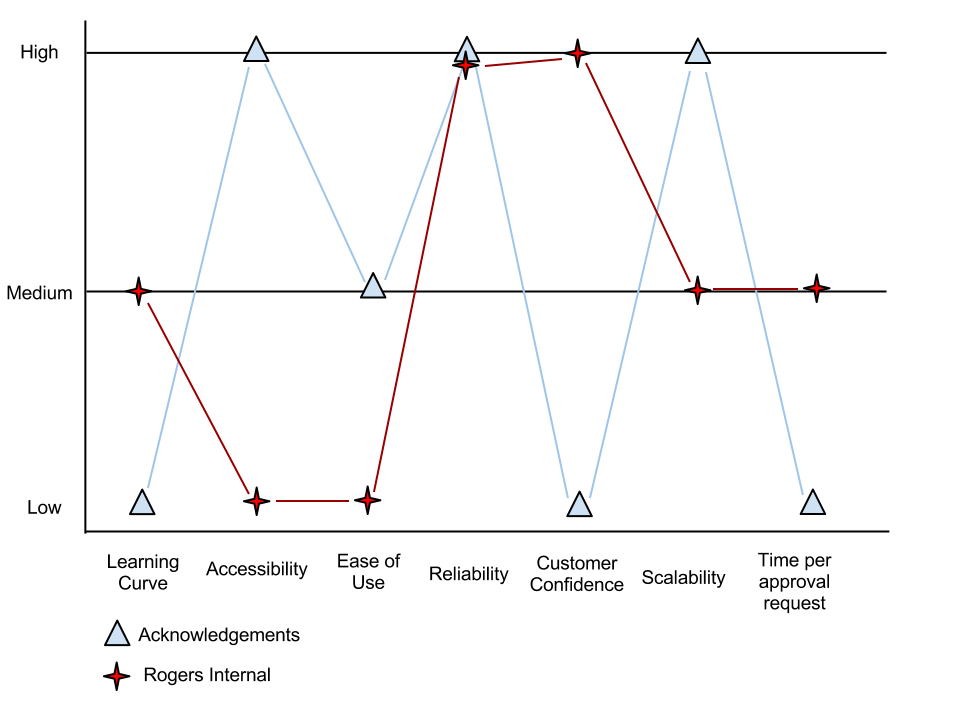
\includegraphics[width=150mm]{images/MSCI454-ValueCurve.png}
\caption{Value Curve}
\label{valuecurve}
\end{figure}

\subsection{Go-to-Market Strategy}

Our go-to-market strategy involves seeking initial clients in August of 2013. The entire development plan from the early stages to the revenue-earning phase is detailed in Figure \ref{growthCycle}.

\begin{figure}[ht!]
\centering
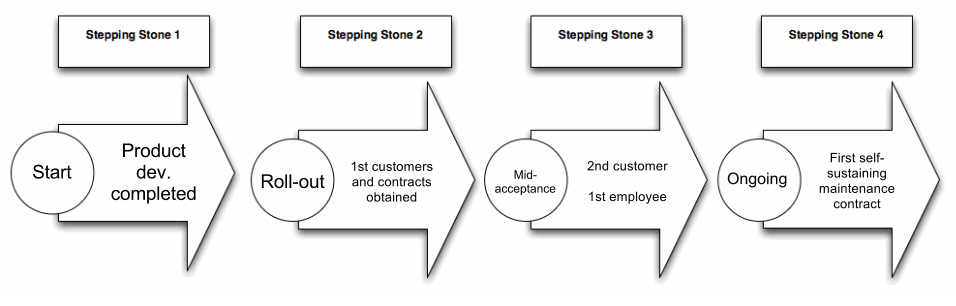
\includegraphics[width=150mm]{images/MSCI454-SteppingStones.png}
\caption{Growth Cycle}
\label{growthCycle}
\end{figure}

{\it Acknowledgements} will enter the product development stage by early May 2013. With an experienced founding team, an initial release of {\it Acknowledgements} will be ready by late-August 2013.

An intial beta version of {\it Acknowledgements} will enter on-site client testing phases by the end of August 2013. Our next set of customers will be obtained by end-of-year 2013.

Once a solid customer base is established, {\it Acknowledgements} will enter the ongoing growth phase. Self-sustaining maintenance contracts will be the main source of revenue for the company, and further funding will not be required.

% \subsection{Hiring Cycle}

% Once {\it Acknowledgements} has achieved its {\bf Mid-Acceptance} milestone presented in figure \ref{growthCycle} we will hire our first employee. As our second customer base is acquired, the extra work will require the additional employee to help maintain the maintenance contracts.

% As {\it Acknowledgements} grows to its {\bf Ongoing} milestone, it will be time to hire new sales staff. Maintenance contracts will make up the majority of our work base, and new clients need to be acquired. At this point within our first year, a single sales staff will represent {\it Acknowledgements} on the market. It will be expected that this staff bring in more clients. 

\subsection{Customer Retention}
{\it Acknowledgements} will have high customer retention not only because it will offer an exception product, but also because of the large cost to a company to switch an application which is so tightly tied into that company's operations. One of the most significant challenges in acquiring a client will eventually benefit {\it Acknowledgements} in terms of client retention. Research shows that companies tend to invest in a particular approval software solution, and then stick with it. This is exemplified by the problem we are trying to address: Companies have blindly stuck with their unacceptable approval software for years because the hassle of changing was undesirable.

\subsection{Target Customers}
Our target customers are the major Canadian general contractors. The approval process is entrenched in their company's work flow and it is often the case that the software they use for this task is many years outdated. 

Our largest target customers include many of the members of the Canadian Construction Association including:

\begin{enumerate}
  \item AECON Buildings
  \item Hamilton-Halton Construction Association
  \item Infrastructure Ontario
  \item PCL Constructors Inc.
  \item Pennecon Ltd.
\end{enumerate}

There are hundreds of general contracting firms across Canada, each of which is a viable client. While initially {\it Acknowledgements} will be targeted at the Canadian construction industry, it will quickly expand internationally once a client base is established. Industry regulations and other legal requirements will be significant considerations when expanding outside of Canada.